% =============================================================================
% File        : poster.tex
% Project     : The Knowledge Lifecycle of Large Language Models
% Purpose     : A0 portrait conference poster, carrying the five lifecycle
%               colors used by the paper, the deck, the repository, the demo.
% Authors     : Amey Thakur, Sarvesh Talele
% Repository  : https://github.com/Amey-Thakur/LLM-KNOWLEDGE-LIFECYCLE
% License     : CC BY 4.0
% =============================================================================
%
% A0 portrait is 84.1 x 118.9 cm. The class margin leaves a measure of 82.5 cm
% and about 116 cm of height, both measured off the rendered PDF.
%
% Every figure is drawn in arbitrary units inside \resizebox{\linewidth}{!}{...},
% which scales the type along with the picture. Each is therefore drawn at a
% natural width of (container / 1.4), so all of them land on the same 1.4x scale
% and every label sets at about 35 pt against 25 pt body text.
%
%   full width  81.0 cm  ->  58.0 units      0.34 column  25.5 cm  ->  18.2
%   0.58 column 45.5 cm  ->  32.5 units      0.32 column  24.0 cm  ->  17.1
%   0.42 column 32.5 cm  ->  23.2 units
%
% Each lane plan is set so the rightmost element lands on the right edge of its
% natural width, leaving no white down the side of the block.
%
% Overlap is prevented two ways. Lists, callouts and code samples are LaTeX
% boxes, which cannot overlap. Where geometry is needed, every text node carries
% an explicit text width and its clearance is worked from the average character
% advance of 0.45 units at body size. The rendered PDF is then checked for
% intersecting text boxes.
%
% tikzposter silently drops anything past the bottom of the page, so the lowest
% ink in the output is measured rather than assumed. An empty block title still
% reserves its full height; the negative leads below cancel it.
%
% Blocks in a row are independent. The coverage statistic sits in the left column
% of row 1 and the replication note closes the right column of row 3, so the two
% rows come out level.
%
% Reading order runs down the page, not down each column: problem, framework,
% evidence, then the contributions and how to check them.
%
% hyperref is absent: tikzposter applies its theme inside a group and hyperref
% fails there either side of \usetheme. At A0 a link buys nothing, so URLs are
% plain text.

\documentclass[25pt, a0paper, portrait, blockverticalspace=13mm, colspace=18mm,
               subcolspace=8mm]{tikzposter}

\usepackage{amsmath}
\usepackage{amssymb}
\usepackage{tikz}
\usetikzlibrary{arrows.meta, positioning, calc, decorations.pathreplacing}

% Removes the "LaTeX TikZposter" mark the class prints over the footer.
\tikzposterlatexaffectionproofoff

% Sans throughout, body and figures alike, so the page reads as one document.
\renewcommand{\familydefault}{\sfdefault}

% --- the five lifecycle colors, identical across every surface ---------------
\definecolor{acquire} {HTML}{4A7FD4}
\definecolor{store}   {HTML}{2A9D8F}
\definecolor{retrieve}{HTML}{E08A2E}
\definecolor{update}  {HTML}{D05353}
\definecolor{forget}  {HTML}{8F5FB8}
\definecolor{ink}     {HTML}{1A1A1C}
% Darker than the screen palette: the poster is printed, not backlit.
\definecolor{muted}   {HTML}{4A4A55}
\definecolor{hairline}{HTML}{C8CAD2}
\definecolor{ok}      {HTML}{2E7D32}
\definecolor{panel}   {HTML}{F4F4F7}

\usetheme{Default}
\usebackgroundstyle{Empty}
\usetitlestyle{Empty}

% Minimal rules under the block title. A custom style cannot be used: its rule
% dereferences the blocktitle node, which an empty title never creates.
\useblockstyle{Minimal}

\colorlet{backgroundcolor}{white}
\colorlet{framecolor}{acquire}
\colorlet{blocktitlebgcolor}{white}
\colorlet{blocktitlefgcolor}{ink}
\colorlet{blockbodybgcolor}{white}
\colorlet{blockbodyfgcolor}{ink}

% Ragged right with hyphenation off. Justified setting in a 25 cm column at this
% size breaks words across lines, and the poster is read standing up.
\newcommand{\bodyset}{%
  \raggedright\hyphenpenalty=10000\exhyphenpenalty=10000\relax}

% -----------------------------------------------------------------------------
% The identity band. It opens and closes the page at full weight and divides the
% header from the content at a third of that weight, so the divider reads as a
% rule inside a frame rather than as a repeating pattern.
%
% The band is drawn 58 units wide and scaled to the width the caller passes,
% which must be the 82.5 cm measure: \textwidth is the 84.1 cm paper width and
% runs the band off the right edge of the sheet.
%
% The bounding box is stated outright. Without it a stray node stretches the
% picture, and since \resizebox fixes the width of the whole box the visible
% part then shrinks inside a nominally full-width band.
% -----------------------------------------------------------------------------
\newcommand{\stageband}[2]{%  #1 = target width, #2 = height in band units
  \resizebox{#1}{!}{%
    \begin{tikzpicture}
      \foreach \c/\a/\b in {acquire/0/11.6, store/11.6/23.2, retrieve/23.2/34.8,
                            update/34.8/46.4, forget/46.4/58}
        {\fill[\c] (\a, 0) rectangle (\b, #2);}
      \useasboundingbox (0, 0) rectangle (58, #2);
    \end{tikzpicture}}%
}

% The three bands are drawn from two boxes of different measure: the title at
% 82.5 cm and the footer block at 80.9 cm, indented 0.8 cm further in. \bandw is
% captured once from the title, every band is drawn at that width, and each is
% shifted by half the difference so all three sit on the same page axis. The
% enclosing \makebox is the local measure, so the overhang is not overfull.
\newlength{\bandw}
% A fallback, so that a band is never asked to scale itself to zero width if the
% title is ever moved after something that draws one.
\AtBeginDocument{\ifdim\bandw=0pt \global\bandw=\textwidth\fi}
\newcommand{\atbandwidth}[1]{%
  \noindent\makebox[\linewidth][l]{%
    \hspace*{\dimexpr(\linewidth-\bandw)/2\relax}#1}%
}

% -----------------------------------------------------------------------------
% A callout: an accent rule, a tinted panel, and text that wraps inside it.
% A self-sizing node, so the panel is exactly as tall as its content. The 10 mm
% inner padding clears the 6 mm accent rule by 4 mm.
% -----------------------------------------------------------------------------
\newlength{\calloutwidth}
\newcommand{\callout}[2]{%  #1 = accent color, #2 = content
  \setlength{\calloutwidth}{\dimexpr\linewidth-20mm\relax}%
  \noindent\begin{tikzpicture}
    \node[fill=panel, text width=\calloutwidth, inner sep=10mm,
          align=left, anchor=north west] (c) at (0,0) {#2};
    \fill[#1] (c.south west) rectangle ([xshift=6mm]c.north west);
  \end{tikzpicture}%
}

% An author: portrait, name, city, ORCID. Both cards come from this macro at the
% same width, so the pair is symmetric about the page center by construction.
% The 10.2 cm measure holds the widest line, the ORCID at about 9.9 cm.
\newcommand{\authorcard}[4]{%  #1 portrait, #2 name, #3 city, #4 ORCID
  \begin{minipage}[c]{3.8cm}\includegraphics[width=3.6cm]{#1}\end{minipage}%
  \hspace{6mm}%
  \begin{minipage}[c]{10.2cm}\raggedright
    {\fontsize{36}{42}\selectfont\bfseries\color{ink} #2\par}
    \vspace{1mm}
    {\fontsize{26}{32}\selectfont\color{muted} #3\par}
    {\fontsize{24}{30}\selectfont\color{muted} ORCID #4\par}
  \end{minipage}%
}

\title{Probability Is Not an Answer}
\author{Amey Thakur \quad Sarvesh Talele}
\institute{Independent Research}

\settitle{
  \centering
  % Captured here, at the top of the title, where \linewidth is the 82.5 cm
  % measure. Every band on the page is then drawn at this one width. The
  % assignment is global because tikzposter typesets the title inside a node,
  % and a local length would revert before the footer band is reached.
  \global\bandw=\linewidth\relax
  % The class leaves 1.30 cm above this band. With the air around the author
  % strip and the divider pulled in below it, the page carries 4.99 cm of slack,
  % so this lead puts 2.50 cm at the top and leaves 2.49 cm at the foot.
  \vspace*{12mm}
  \atbandwidth{\stageband{\bandw}{0.9}}
  \vspace{8mm}

  % Scaled to the measure rather than set at a point size, so the title holds
  % one line and its size follows from the width.
  \resizebox{\linewidth}{!}{\bfseries\color{ink}%
    Probability Is Not an Answer}
  \vspace{7mm}

  {\fontsize{40}{50}\selectfont\color{muted}
   A model holds two memories. Which one comes out is not a question of size.\par}
  % Equal air above and below, so the two faces read as their own band rather
  % than as a caption on the subtitle. The \par after the cards is required:
  % without it the \vspace lands inside the paragraph as a \vadjust and the
  % interline glue absorbs almost all of it.
  \vspace*{18mm}

  \authorcard{amey-circle.png}{Amey Thakur}{Toronto, Canada}{0000-0001-5644-1575}%
  \hspace{22mm}%
  \authorcard{sarvesh-circle.png}{Sarvesh Talele}{Mumbai, India}{0009-0002-0818-461X}%
  \par
  \vspace*{18mm}

  % A third of the weight of the opening and closing bands: enough to divide the
  % header from the content, not enough to compete with them.
  \atbandwidth{\stageband{\bandw}{0.3}}
  % The class leaves 5.06 cm between this rule and the first block title, which
  % reads as a break rather than as a division. This pulls it back to about
  % 2.9 cm, so the divider sits with the content it introduces.
  \vspace*{-18mm}
}

\begin{document}

\maketitle[width=\textwidth]

% =============================================================================
% ROW 1  |  the problem, and the framework that answers it
% =============================================================================
\begin{columns}
\column{0.42}
\colorlet{framecolor}{update}
\block{The problem}{\bodyset
  How a language model handles a fact is studied by \textbf{five separate
  communities} that rarely cite one another.
  \vspace{6mm}

  % Full-measure rows rather than a swatch and a word, so the tinted band carries
  % the eye to the right edge of the column. Natural width 23.2 units against a
  % 32.5 cm column: the 1.4x scale. The longest name is 13.5 units and the text
  % starts at 1.5, so nothing reaches the 23.2 edge.
  \resizebox{\linewidth}{!}{%
  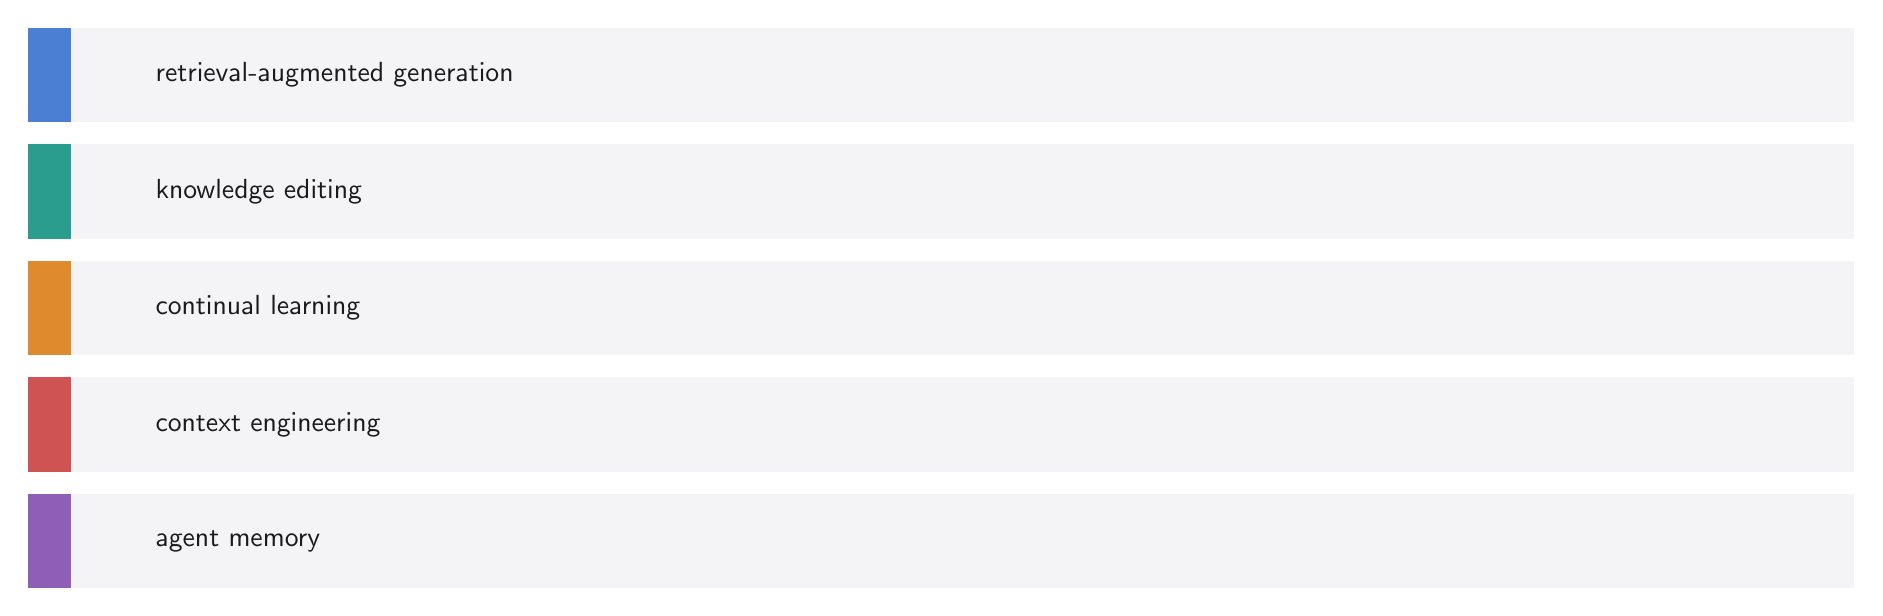
\begin{tikzpicture}
    \foreach \c/\n [count=\i from 0] in
      {acquire/retrieval-augmented generation, store/knowledge editing,
       retrieve/continual learning, update/context engineering,
       forget/agent memory}
      {\fill[panel] (0, -\i*1.48) rectangle (23.2, -\i*1.48 + 1.20);
       \fill[\c]    (0, -\i*1.48) rectangle (0.55, -\i*1.48 + 1.20);
       \node[anchor=west, text=ink] at (1.5, -\i*1.48 + 0.60) {\n};}
    \useasboundingbox (0, -5.92) rectangle (23.2, 1.20);
  \end{tikzpicture}}
  \vspace{5mm}

  Each has its own benchmarks, and each passes them. A system can pass
  \textbf{all five} and still fail, because nothing tests what happens
  \textbf{between} them.
  \vspace{7mm}

  \callout{acquire}{Across \textbf{20 representative papers}, the median work
    covers \textbf{two} of the five stages. The boundaries are where deployment
    breaks.}
}

\column{0.58}
\colorlet{framecolor}{acquire}
\block{The framework}{\bodyset
  A fact passes through five stages. Naming them as one lifecycle is what makes
  the boundaries between them visible.
  \vspace{7mm}

  % Natural width 32.6 units against a 45.5 cm column: the 1.4x figure scale.
  % Boxes are 5.5 wide on a 6.7 pitch. Each caption is confined to a 5.5 unit
  % text width, so the 1.2 unit gutter between boxes is never encroached on.
  \resizebox{\linewidth}{!}{%
  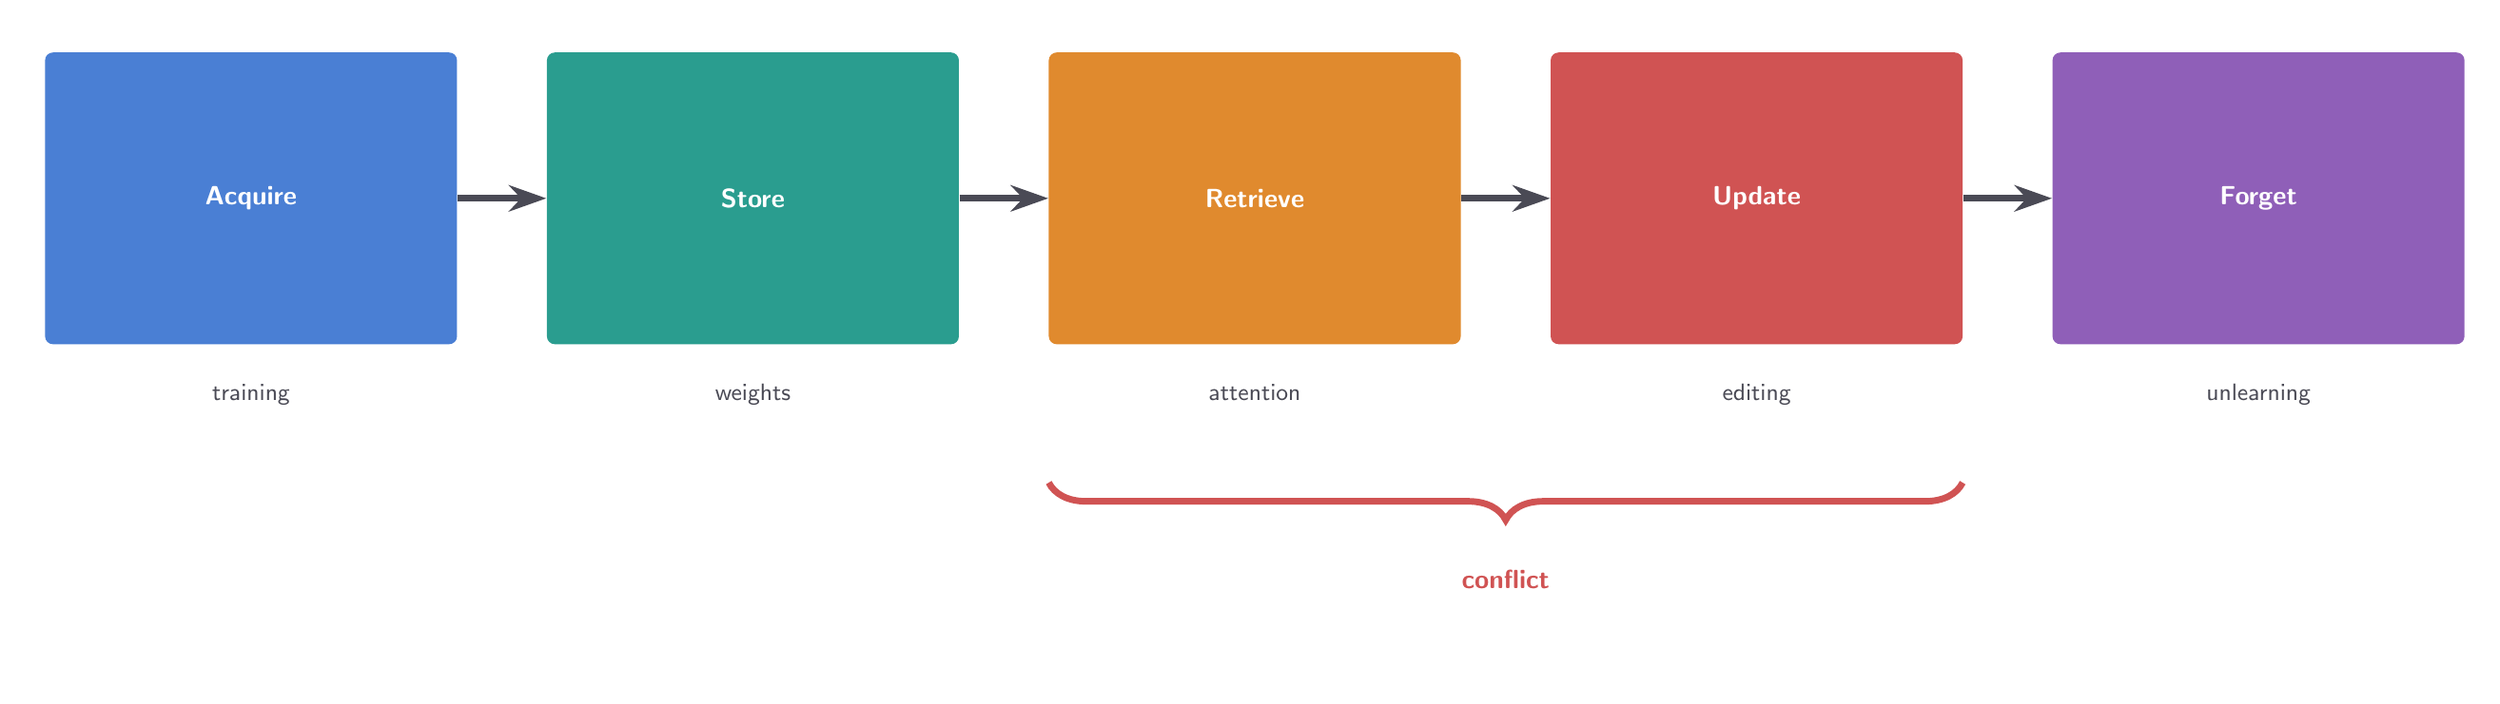
\begin{tikzpicture}[
    lcbox/.style={rounded corners=3pt, minimum width=5.5cm, minimum height=3.9cm,
                  text=white, font=\bfseries, align=center},
    lccap/.style={text=muted, font=\small, text width=5.5cm, align=center},
    lcflow/.style={-{Stealth[length=5mm, width=3.5mm]}, line width=2.5pt, muted}
  ]
    \node[lcbox, fill=acquire]  (a) at (0,0)    {Acquire};
    \node[lcbox, fill=store]    (s) at (6.7,0)  {Store};
    \node[lcbox, fill=retrieve] (r) at (13.4,0) {Retrieve};
    \node[lcbox, fill=update]   (u) at (20.1,0) {Update};
    \node[lcbox, fill=forget]   (f) at (26.8,0) {Forget};

    \draw[lcflow] (a) -- (s);
    \draw[lcflow] (s) -- (r);
    \draw[lcflow] (r) -- (u);
    \draw[lcflow] (u) -- (f);

    \node[lccap, below=4mm of a] {training};
    \node[lccap, below=4mm of s] {weights};
    \node[lccap, below=4mm of r] {attention};
    \node[lccap, below=4mm of u] {editing};
    \node[lccap, below=4mm of f] {unlearning};

    % The conflict spans two stages, so it is braced beneath both rather than
    % labelled on the arrow between them. Captions bottom out near y = -3.35,
    % the brace sits at -3.8 and its label at -5.1.
    \draw[update, line width=2.5pt, decorate,
          decoration={brace, mirror, amplitude=5mm}]
      (10.65, -3.8) -- (22.85, -3.8);
    \node[text=update, font=\bfseries] at (16.75, -5.1) {conflict};
    \useasboundingbox (-3.0, -6.4) rectangle (29.6, 2.3);
  \end{tikzpicture}}
  \vspace{7mm}

  % A callout rather than running text, so the two columns of this row end level
  % and the sentence handing off to the finding carries its weight.
  \callout{update}{The failure below sits between
    \textcolor{retrieve}{\textbf{Retrieve}} and
    \textcolor{update}{\textbf{Update}}: the document arrives, and nothing
    tells the model which copy of the fact to trust.}
}
\end{columns}

% =============================================================================
% ROW 2  |  the finding, full width, the largest figure on the page
% =============================================================================
\colorlet{framecolor}{update}
\block{The finding}{\bodyset
  Give each model a fact it already holds, then a document asserting something
  else. \textbf{864 forward passes}: six models, 24 counterfactual probes, three
  phrasings, with and without the document. Read at the \textbf{rank} of the
  answer, which is what the model would actually say.
  \vspace{6mm}

  % Natural width 58 units against the 81 cm measure: the 1.4x figure scale.
  % Six groups on a 9.6 pitch, each holding two 3.0-wide bars with a 1.3 gutter,
  % so a group spans 0.5 to 7.8 of its own cell and the pair never touches its
  % neighbour. Bars are 0.058 units per percentage point, so a full 100% stands
  % 5.8 units and the value label above it clears the legend at y = 7.6.
  \resizebox{\linewidth}{!}{%
  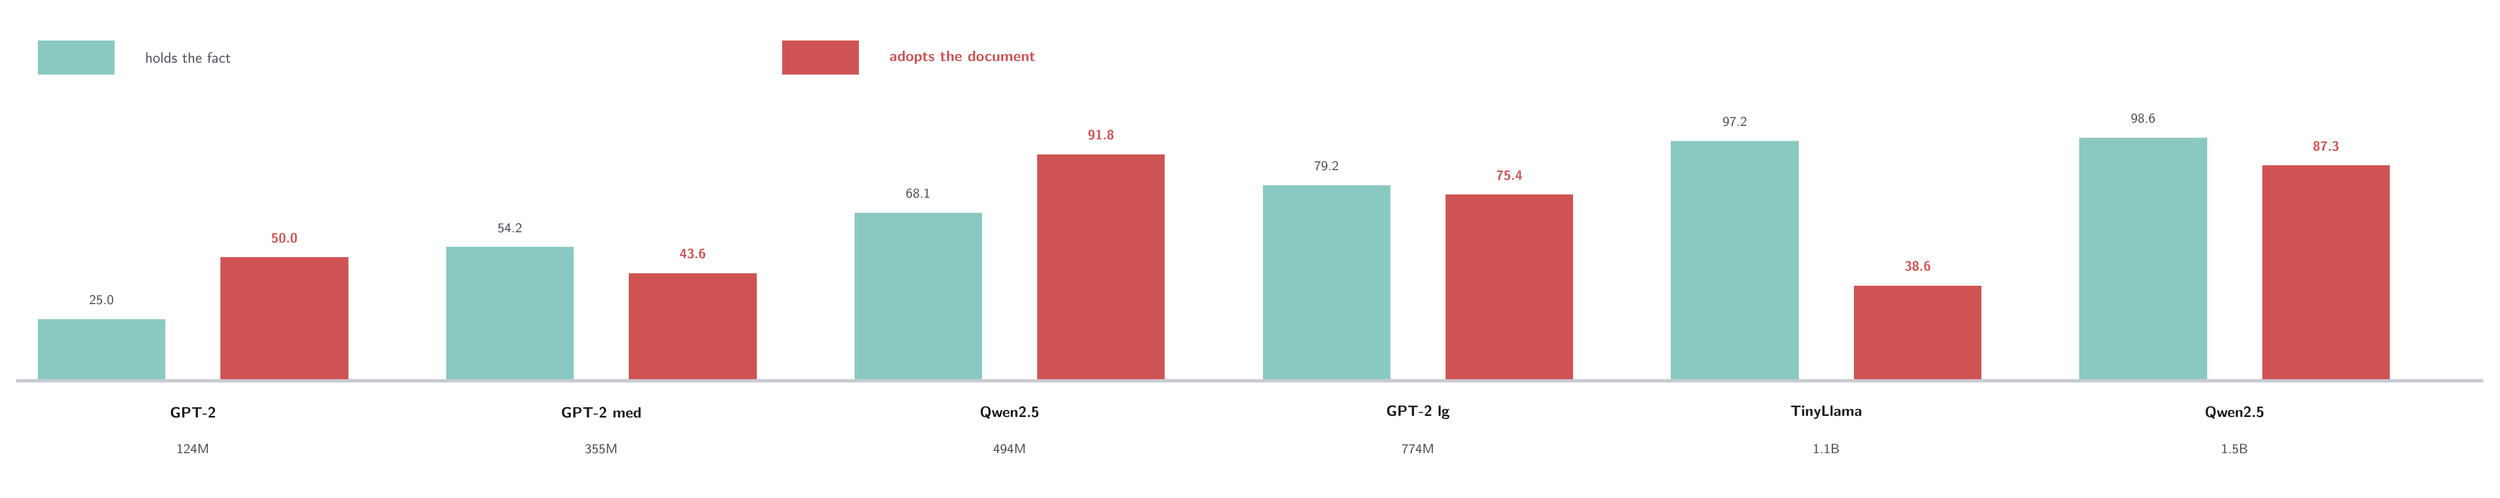
\begin{tikzpicture}
    % \par is a TeX primitive and must never be used as a loop variable.
    \foreach \x/\name/\psize/\knows/\adopt [count=\i from 0] in {%
      0/GPT-2/124M/25.0/50.0,
      1/GPT-2 med/355M/54.2/43.6,
      2/Qwen2.5/494M/68.1/91.8,
      3/GPT-2 lg/774M/79.2/75.4,
      4/TinyLlama/1.1B/97.2/38.6,
      5/Qwen2.5/1.5B/98.6/87.3}
      {\pgfmathsetmacro{\gx}{\x*9.6}
       \pgfmathsetmacro{\hk}{\knows*0.058}
       \pgfmathsetmacro{\ha}{\adopt*0.058}
       \fill[store!55]  ({\gx+0.5},0) rectangle ({\gx+3.5},\hk);
       \fill[update]    ({\gx+4.8},0) rectangle ({\gx+7.8},\ha);
       \node[text=muted, font=\small] at ({\gx+2.0},{\hk+0.45}) {\knows};
       \node[text=update, font=\bfseries\small] at ({\gx+6.3},{\ha+0.45}) {\adopt};
       \node[text=ink, font=\bfseries] at ({\gx+4.15},-0.75) {\name};
       \node[text=muted, font=\small]  at ({\gx+4.15},-1.6) {\psize};}

    \draw[hairline, line width=2pt] (0,0) -- (58,0);

    % legend, top left, clear of the tallest bar at 5.8
    \fill[store!55] (0.5, 7.2) rectangle (2.3, 8.0);
    \node[anchor=west, text=muted] at (2.9, 7.6) {holds the fact};
    \fill[update]   (18.0, 7.2) rectangle (19.8, 8.0);
    \node[anchor=west, text=update, font=\bfseries] at (20.4, 7.6)
      {adopts the document};
    \useasboundingbox (0, -2.4) rectangle (58, 8.6);
  \end{tikzpicture}}
  \vspace{7mm}

  \callout{update}{%
    {\Large\bfseries Holding a fact scales with size. \textcolor{update}{Using
     the document does not.}\par}
    \vspace{5mm}
    {\color{muted}Knowing the answer climbs monotonically with parameter count,
     $25.0$ to $98.6$ per cent, with no inversion anywhere. What the model then
     does with a contradicting document follows no such order: TinyLlama holds
     the fact $97.2$ per cent of the time and defers least of the six, while
     Qwen2.5-0.5B, a third its size, defers $91.8$ per cent.\par}}
}

% =============================================================================
% ROW 3  |  the two contributions, and how to check them
% =============================================================================
\begin{columns}
\column{0.34}
\colorlet{framecolor}{retrieve}
\block{Probability is not an answer}{\bodyset
  The probability a model puts on an answer and the answer it gives are
  \textbf{different quantities}. Mass is spread over tens of thousands of
  tokens, so the answer has only to be ranked first, not to be large.
  \vspace{8mm}

  % Natural width 18.2 units against a 25.5 cm column: the 1.4x figure scale.
  % One stacked bar, 4.0 tall, split at 332/432 and then within that at 69/332.
  % Every label sits outside the bar, so none can be clipped by its own fill.
  \resizebox{\linewidth}{!}{%
  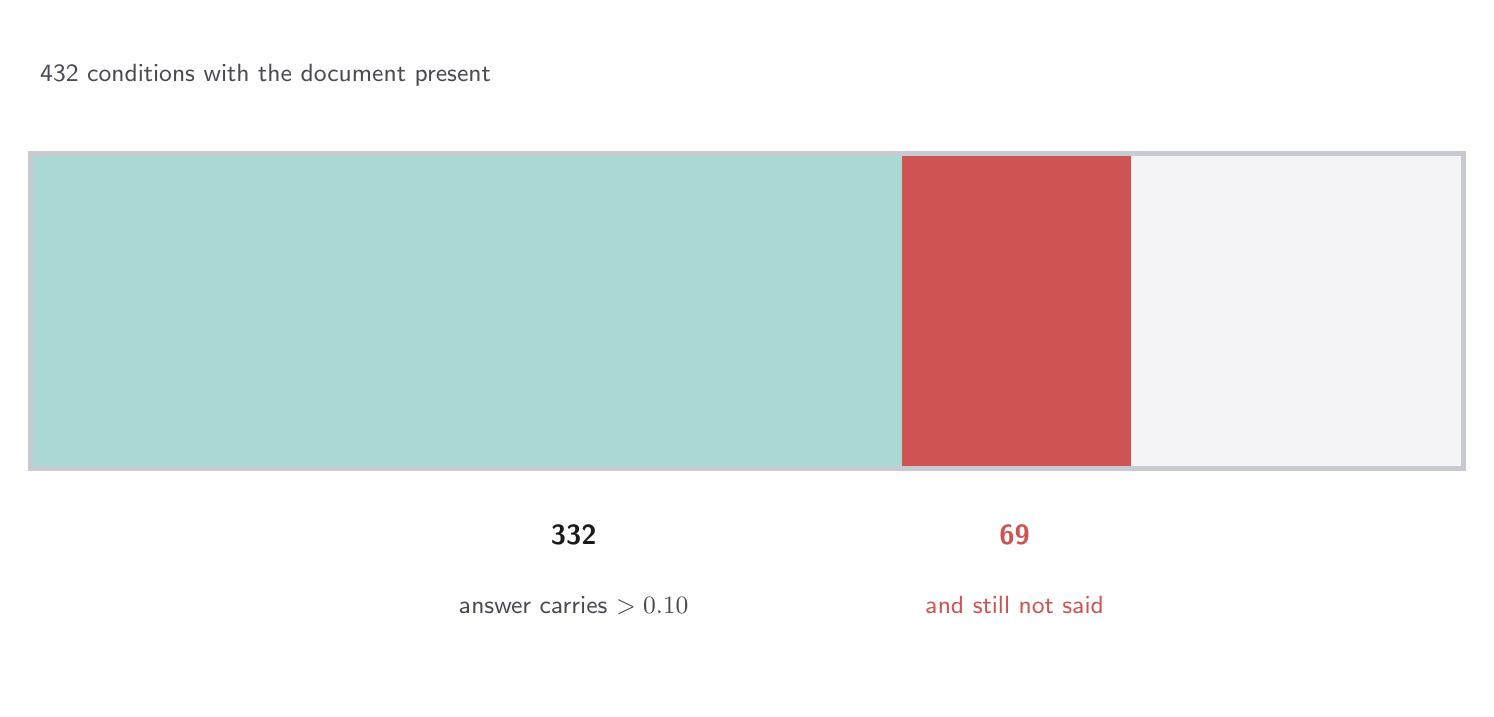
\begin{tikzpicture}
    \fill[panel]      (0,    0) rectangle (18.2, 4.0);
    \fill[store!40]   (0,    0) rectangle (13.98, 4.0);
    \fill[update]     (11.07, 0) rectangle (13.98, 4.0);
    \draw[hairline, line width=2pt] (0,0) rectangle (18.2,4.0);

    \node[anchor=west, text=muted, font=\small] at (0, 5.0)
      {432 conditions with the document present};
    \node[anchor=north, text=ink, font=\bfseries] at (6.9, -0.6) {332};
    \node[anchor=north, text=muted, font=\small] at (6.9, -1.5)
      {answer carries $>0.10$};
    \node[anchor=north, text=update, font=\bfseries] at (12.5, -0.6) {69};
    \node[anchor=north, text=update, font=\small] at (12.5, -1.5)
      {and still not said};
    \useasboundingbox (0, -2.8) rectangle (18.2, 5.6);
  \end{tikzpicture}}
  \vspace{8mm}

  In \textbf{20.8\%} of the conditions where the in-context answer carries real
  probability, it is \textbf{still not what the model says}. Recording the rank
  costs \textbf{one comparison}.
}

\column{0.34}
\colorlet{framecolor}{store}
\block{A correction}{\bodyset
  An earlier version of this work reported that no model answers a
  drug-withdrawal probe correctly under any phrasing. \textbf{That claim was
  false}, and how it failed is why this poster exists.
  \vspace{8mm}

  \callout{update}{The script behind it recorded only the \textbf{surprisal} of
    the expected answer. It never recorded that answer's \textbf{rank}, nor
    which token the model put first, so it could not have tested the claim it
    was cited for.}
  \vspace{8mm}

  Re-run with rank recorded, \textbf{three of the six} models rank the corrected
  answer first under two of the three phrasings.
  \vspace{6mm}

  A second defect was structural: those probes were \textbf{real-world updates},
  and the withdrawal predates every model's training data, so \textbf{no
  conflict existed to resist}.
}

\column{0.32}
\colorlet{framecolor}{forget}
\block{Reproduce it}{\bodyset
  Every number on this poster comes from \textbf{one deterministic script}.
  Nothing is sampled, so the digits come out identical on any machine.
  \vspace{8mm}

  \callout{forget}{\ttfamily
    pip install torch transformers\par
    \vspace{4mm}
    python counterfactual\_update.py}
  \vspace{8mm}

  Six models in float32 on \textbf{CPU}, about twenty minutes on a laptop, so
  the digits do not depend on an accelerator's arithmetic.
  \vspace{7mm}

  Every figure here is \textbf{generated} from the measurement, never typed. The
  earlier version quoted a number its own code had never produced.
  \vspace{7mm}

  \callout{muted}{\color{muted}The probes are all national capitals, so this is
    about one kind of fact; numeric and temporal facts are untested.}
}

\end{columns}

% =============================================================================
% FOOT  |  where to find the work, then the identity band closing the page
% =============================================================================
\colorlet{framecolor}{hairline}
\block{}{
  % An empty block title still reserves its full height in tikzposter, 4.8 cm of
  % white that pushes the closing band off the bottom of the page, where the
  % class drops it silently. The lead below cancels it. The rebuilt evidence row
  % is taller than the one it replaced, so this now cancels the title height
  % outright rather than most of it: at -30 mm the three bays' headings printed
  % and their addresses fell past the page edge.
  \vspace*{-48mm}
  \textcolor{hairline}{\rule{\linewidth}{2pt}}
  \vspace{6mm}

  % Three bays of equal width and equal gutters, so the row is symmetric about
  % the page center by construction. A bay is 25.9 cm and the longest address
  % sets to 22.7 cm, so every URL holds one line.
  \noindent
  \begin{minipage}[t]{0.32\linewidth}\centering
    {\bfseries Paper and code}\par\vspace{3mm}
    {\small\color{muted} github.com/Amey-Thakur/LLM-KNOWLEDGE-LIFECYCLE\par}
  \end{minipage}\hfill
  \begin{minipage}[t]{0.32\linewidth}\centering
    {\bfseries Live demonstration}\par\vspace{3mm}
    {\small\color{muted} huggingface.co/spaces/ameythakur/llm-knowledge-lifecycle\par}
  \end{minipage}\hfill
  \begin{minipage}[t]{0.32\linewidth}\centering
    {\bfseries ORCID}\par\vspace{3mm}
    {\small\color{muted} Thakur 0000-0001-5644-1575 \quad Talele 0009-0002-0818-461X\par}
  \end{minipage}
  \vspace{8mm}

  % Far enough below the bays to read as its own line, not as a third line of
  % the middle bay.
  {\centering\small\color{muted} Released under CC BY 4.0\par}
  \vspace{6mm}

  \atbandwidth{\stageband{\bandw}{0.9}}
}

\end{document}
